\chapter{The ATLAS Experiment}
\label{sec:ATLAS}

The ATLAS detector is one of the two general purpose detectors on LHC, and is designed for probing for p-p and A-A collisions.
This detector represents the work of a large collaboration of several thousand physicists, engineers, technicians,
and students over a period of fifteen years of dedicated design, development, fabrication, and installation.
There are several fields in which the resarches are currently going in ATLAS collaboration, including Z and W boson decay, search for Higgs boson,
supersymmetry, study on B-mesons, and others. This broad spectrum of researches makes high demands on the detector's complexity and the precision 
of the different sub-systems.

\section{Physics requirements and detector overview}
\label{sec:ATLAS_overview}
The ATLAS detector has a cylindric shape, it is aligned along the beam line with the center situated at the interaction point.
The coordinate system that is used to describe the detector follows its natural geometry. the interaction point is taken as an origin,
while the $z$ axis is put along the beam pipe, making the $x$-$y$ plane transverse. The positive $x$-axis is defined to be pointing to the center
of the LHC ring, and positive $y$-axis is defined to be pointing upwards. The direction on the $z$-axis is picked such as to form a right-handed coordinate system.
The azimuthal angle $\varphi$ is measured as usual around the beam axis, and the polar angle $\theta$ is the angle from the beam axis. The rapidity $y$ and pseudorapidity $\eta$
are calculated using the standard equations:

\disn{}{
y = \frac{1}{2} \log \left(\frac{E+p_z}{E-p_z}\right),
\nom}

\disn{}{
\eta = - \log (\tan (\frac{\theta}{2})),
\nom}

\begin{figure}
\center{
\includegraphics[width=1.0\textwidth]{figures/ATLAS_overview.eps}
\caption{Overview of the ATLAS detector, with all the major sub-systems and the human-sized scale figures~\cite{lib:ATLASdet}.}
\label{fig:ATLAS_overview}}
\end{figure}

The overview of the ATLAS detector is shown on the Fig.~\ref{fig:ATLAS_overview}. The main detector sub-systems can be seen there: the innermost is the tracker, then goes the EM calorimeters, then the hadronic calorimeters, and finally the muon spectrometers. There is also a magnet system, which is not a detector by itself, but is essential to the functioning of the whole system. All of the sub-detectors are briefly described below.

\begin{itemize}
\item The tracker (also called "the inner detector") records the tracks of the particles and is used to determine the charge and transverse momentum.
\item The EM calorimeters identify and measure the energy of EM particles: electrons, positrons and photons.
\item The hadronic calorimeters measure the energy of hadrons.
\item The muon spectrometers identify and measure the energy, momentum and charge of the muons.
\end{itemize}



\section{Tracking}
\label{sec:ATLAS_tracker}

Because of the very high number of the events per second, the density of the tracks inside the inner detector is also very high. We are getting approximately 1000 particles
from the collision point every 25 ns within the central eta region which we need to record. To achieve the needed momentum and vertex resolution, high-precision measurements must be made with fine detector granularity. The tracker of the ATLAS detector consists of pixel and silicon microstrip (SCT) trackers, and the Transition Radiation Tracker (TRT). Combined they provide these features.

\begin{figure}
\center{
\includegraphics[width=1.0\textwidth]{figures/ATLAS_tracker.eps}
\caption{Overview of the ATLAS tracker. The SCT, TRT and pixel detectors are shown there~\cite{lib:ATLASdet}.}
\label{fig:ATLAS_tracker}}
\end{figure}

The layout of the tracker is illustrated in Fig.~\ref{fig:ATLAS_tracker}. Its
basic parameters are summarised in Tab.~\ref{tab:ATLAS_tracker}. The magnetic field with the intencity of $2T$ generated by the central solenoid covers most of the tracker: it extends over a length of $5.3 m$ with a diameter of $2.5 m$. The precision tracking detectors (pixels and SCT) cover the region
$|\eta|<2.5$. As can be seen on the picture, in the central area they are arrengad in concentric cylinders along the beam axis, while in the end-cap regions they are arranged in form of discs perpendicular to the beam. The highest granularity is achieved around the interaction point using silicon pixel detectors. The pixel layers are
segmented in $\varphi$ and $z$ with typically three pixel layers crossed by each track. All pixel sensors
are identical and have a minimum pixel size in $R-\varphi \times z-\varphi$ of $50 \times 400 \mu m^2$. The intrinsic accuracies
in the central region are $10 \mu m$ $(\varphi)$ and $115$ $\mu m$ $(z)$ and in the end-cap regions are $10 \mu m$ $(\varphi)$ and $115 \mu m$ $(R)$.
The pixel detector has approximately 80.4 million readout channels. For the SCT, eight strip layers
(four space points) are crossed by each track. In the central region, this detector uses small-angle
($40 mrad$) stereo strips to measure both coordinates, with one set of strips in each layer parallel to
the beam direction, measuring $R-\varphi$. They consist of two $6.4 cm$ long daisy-chained sensors with
a strip pitch of $80 \mu m$. In the end-cap region, the detectors have a set of strips running radially and
a set of stereo strips at an angle of $40 mrad$. The mean pitch of the strips is also approximately
$80 \mu m$. The intrinsic accuracies per module in the barrel are $17 \mu m$ $(\varphi)$ and $580 \mu m$ $(z)$ and in
the disks are $17 \mu m$ $(\varphi)$ and $580 \mu m$ $(R)$. The total number of readout channels in the SCT is
approximately 6.3 million.

\begin{table}
\centering
\begin{tabular}{ll | r@{$<$}c@{$<$}l | r@{$<$}c@{$<$}l} \hline\hline
\multicolumn{2}{l|}{\bf Item} & \multicolumn{3}{c|}{\bf Radial extension (mm)} & \multicolumn{3}{c}{\bf Length (mm)} \\\hline
\multicolumn{2}{l|}{\bf Overall tracker envelope} & $0$&$R$&$1150$ & $0$&$|z|$&$3512$ \\
\multicolumn{2}{l|}{\bf Beam-pipe} & $29$&$R$&$36$ & \multicolumn{3}{c}{}\\\hline
{\bf Pixel} & Overall envelope & $45.5$&$R$&$242$ & $0$&$|z|$&$3092$ \\
3 cylindrical layers & Sensitive barrel & $50.5$&$R$&$122.5$ & $0$&$|z|$&$400.5$ \\
$2*3$ disks & Sensitive end-cap & $88.8$&$R$&$149.6$ & $495$&$|z|$&$650$ \\
\multicolumn{2}{l|}{} & \multicolumn{3}{c|}{} & \multicolumn{3}{c}{}\\
{\bf SCT} & Barrel envelope & $255$&$R$&$549$ & $0$&$|z|$&$805$ \\
 & End-cap envelope & $251$&$R$&$610$ & $810$&$|z|$&$2797$ \\
4 cylindrical layers & Sensitive barrel & $299$&$R$&$514$ & $0$&$|z|$&$749$ \\
$2*9$ disks & Sensitive end-cap & $275$&$R$&$560$ & $839$&$|z|$&$2735$ \\
\multicolumn{2}{l|}{} & \multicolumn{3}{c|}{} & \multicolumn{3}{c}{}\\
{\bf TRT} & Barrel envelope & $554$&$R$&$1082$ & $0$&$|z|$&$780$ \\
 & End-cap envelope & $617$&$R$&$1106$ & $827$&$|z|$&$2744$ \\
73 straw panels & Sensitive barrel & $563$&$R$&$1066$ & $0$&$|z|$&$712$ \\
160 straw panels & Sensitive end-cap & $644$&$R$&$1004$ & $848$&$|z|$&$2710$ \\
\hline\hline
\end{tabular}
\caption{The description of the geomentry of the ATLAS tracker~\cite{lib:ATLASdet}.}
\label{tab:ATLAS_tracker}
\end{table}

A large number of hits (typically 36 per track) is provided by the 4 mm diameter straw tubes
of the TRT, which enables track-following up to $|\eta|=2.0$. The TRT only provides $R-\varphi$ information, for which it has an intrinsic accuracy of $130 \mu m$ per straw. In the central region, the straws are
parallel to the beam axis and are $144 cm$ long, with their wires divided into two halves, approximately at $\eta = 0$. In the end-cap region, the $37 cm$ long straws are arranged radially in wheels. The
total number of TRT readout channels is approximately 351 thousands.

The combination of precision trackers close to interaction point with the TRT at a larger radius gives very
robust pattern recognition and high precision in all $R$ $\varphi$ and $z$ coordinates. The straw hits at the
outer radius contribute significantly to the momentum measurement, since the lower precision per
point compared to the silicon is compensated by the large number of measurements and longer
measured track length.
The inner detector system provides tracking measurements in a range matched by the precision measurements of the electromagnetic calorimeter. The electron identification capabilities
are enhanced by the detection of transition-radiation photons in the xenon-based gas mixture of
the straw tubes. The semiconductor trackers also allow impact parameter measurements and vertexing for heavy-flavour and $\tau$-lepton tagging. The secondary vertex measurement performance is enhanced by the innermost layer of pixels, at a radius of about $5 cm$.


\section{EM calorimeters}
\label{sec:ATLAS_EM_calo}

\begin{figure}
\center{
\includegraphics[width=1.0\textwidth]{figures/ATLAS_calo.eps}
\caption{Overview of the ATLAS EM and hadronic calorimeters.~\cite{lib:ATLASdet}.}
\label{fig:ATLAS_calorimeter}}
\end{figure}


The EM calorimeter is divided into a barrel (central) part ($|\eta| < 1.475$) and two end-cap components
($1.375 < |\eta| < 3.2$), each housed in their own cryostat. The position of the central solenoid in
front of the EM calorimeter demands optimisation of the material in order to achieve the desired calorimeter
performance. As a consequence, the central solenoid and the LAr calorimeter
share a common vacuum vessel, thereby eliminating two vacuum walls. The barrel calorimeter
consists of two identical half-barrels at positive and negative etas, separated by a small gap (4 mm) at z = 0. Each end-cap
calorimeter is mechanically divided into two coaxial wheels: an outer wheel covering the region
$1.375 < |\eta| < 2.5$, and an inner wheel covering the region $2.5 < |\eta| < 3.2$. The EM calorimeter is
a lead-LAr detector with accordion-shaped kapton electrodes and lead absorber plates over its full
coverage. The accordion geometry provides complete $\varphi$ symmetry without azimuthal cracks. The lead thickness in the absorber plates has been optimised as a function of $\eta$ in terms of EM calorimeter performance in energy resolution. Over the region devoted to central analysis ($|\eta| < 2.5$), the
EM calorimeter is segmented in three sections in depth. For the end-cap inner wheel, the calorimeter is segmented in two sections in depth and has a coarser lateral granularity than for the rest of the acceptance.

In the region of $|\eta| < 1.8$, a presampler detector is used to correct for the energy lost by
electrons and photons upstream of the calorimeter. The presampler consists of an active LAr layer
of thickness 1.1 cm in the barrel and 0.5 cm in the end-cap regions.


\section{Hadronic calorimeters}
\label{sec:ATLAS_H_calo}


The hadronic calorimeter consists of the tile calorimeter (the central part) and the hadronic end-cap calorimeter (HEC).

The tile calorimeter is placed directly outside the EM calorimeter envelope. Its
cantral barrel covers the region $|\eta| < 1.0$, and its two extended barrels cover the range $0.8 < |\eta| < 1.7$. It is a
sampling calorimeter using steel as an absorber and scintillating tiles as active material. Both
barrel and extended barrels are divided azimuthally into 64 modules. Radially, the tile calorimeter
extends from an inner radius of 2.28 m to an outer radius of 4.25 m. It is segmented in depth in three
layers, approximately 1.5, 4.1 and 1.8 interaction lengths ($\lambda$) thick for the barrel and 1.5, 2.6, and
3.3 $\lambda$ for the extended barrel. The total detector thickness at the outer edge of the tile-instrumented
region is 9.7 $\lambda$ at $\eta=0$. Two sides of the scintillating tiles are read out by wavelength shifting
fibres into two separate photomultiplier tubes. In $\eta$, the readout cells built by grouping fibres into
the photomultipliers are pseudo-projective towards the interaction region.

The Hadronic End-cap Calorimeter (HEC) consists of two
independent wheels per end-cap, located directly behind the end-cap electromagnetic calorimeter
and sharing the same LAr cryostats. To reduce the drop in material density at the transition between
the end-cap and the forward calorimeter (around $|\eta| = 3.1$), the HEC extends out to $|\eta| = 3.2$,
thereby overlapping with the forward calorimeter. Similarly, the HEC $\eta$ range also slightly overlaps
that of the tile calorimeter ($|\eta| < 1.7)$ by extending to $|\eta| = 1.5$. Each wheel is built from 32
identical wedge-shaped modules, assembled with fixtures at the periphery and at the central bore.
Each wheel is divided into two segments in depth, for a total of four layers per end-cap. The wheels
closest to the interaction point are built from 25 mm parallel copper plates, while those further away
use 50 mm copper plates (for all wheels the first plate is half-thickness). The outer radius of the
copper plates is 2.03 m, while the inner radius is 0.475 m (except in the overlap region with the
forward calorimeter where this radius becomes 0.372 m). The copper plates are interleaved with
8.5 mm LAr gaps, providing the active medium for this sampling calorimeter.

\section{Forward calorimeters}
\label{sec:ATLAS_FCAL}

The forward calorimeter (FCAL) covers the biggest eta range ($3.1 < |\eta| < 4.9$) and combines both EM and hadronic parts.

It is integrated into the end-cap cryostats, as this provides
clear benefits in terms of uniformity of the calorimetric coverage as well as
reduced radiation background levels in the muon spectrometer. In order to reduce the amount of
neutron albedo in the inner detector cavity, the front face of the FCAL is recessed by about 1.2 m
with respect to the EM calorimeter front face. This severely limits the depth of the calorimeter
and therefore calls for a high-density design. The FCAL is approximately 10 interaction lengths
deep, and consists of three modules in each end-cap: the first, made of copper, is optimised for
electromagnetic measurements, while the other two, made of tungsten, measure predominantly the
energy of hadronic interactions. Each module consists of a metal matrix, with regularly spaced
longitudinal channels filled with the electrode structure consisting of concentric rods and tubes
parallel to the beam axis. The LAr in the gap between the rod and the tube is the sensitive medium.
This geometry allows for excellent control of the gaps, which are as small as 0.25 mm in the first
section, in order to avoid problems due to ion buildup.

\section{Muon spectrometers}
\label{sec:ATLAS_muon_chambers}

\begin{figure}
\center{
\includegraphics[width=1.0\textwidth]{figures/ATLAS_muon.eps}
\caption{Overview of the ATLAS muon chambers.~\cite{lib:ATLASdet}.}
\label{fig:ATLAS_muon_chambers}}
\end{figure}


The conceptual layout of the muon spectrometer is shown in Fig.~\ref{fig:ATLAS_muon_chambers}. This system is based on the magnetic
deflection of muon tracks in the large superconducting air-core toroid magnets, instrumented with
separate trigger and high-precision tracking chambers. Over the range $|\eta| < 1.4$, magnetic bending
is provided by the large barrel toroid. For $1.6 < |\eta| < 2.7$, muon tracks are bent by two smaller
end-cap magnets inserted into both ends of the barrel toroid. Over the middle region $1.4 < |\eta| < 1.6$, usually referred
to as the transition region, magnetic deflection is provided by a combination of barrel and end-cap
fields. This magnet configuration provides a field which is mostly orthogonal to the muon trajec-
tories, while minimising the degradation of resolution due to multiple scattering. The anticipated
high level of particle flux has had a major impact on the choice and design of the spectrometer instrumentation,
affecting performance parameters such as rate capability, granularity, ageing
properties, and radiation hardness.

In the barrel region, tracks are measured in chambers arranged in three cylindrical layers
around the beam axis; in the transition and end-cap regions, the chambers are installed in planes
perpendicular to the beam, also in three layers.


\section{Magnet system}
\label{sec:ATLAS_magnets}

\begin{figure}
\center{
\includegraphics[width=1.0\textwidth]{figures/ATLAS_magnet.eps}
\caption{Overview of the ATLAS magnet system.~\cite{lib:ATLASdet}.}
\label{fig:ATLAS_magnets}}
\end{figure}


ATLAS features a unique hybrid system of four large superconducting magnets. This magnetic
system is 22 m in diameter and 26 m in length, with a stored energy of 1.6 GJ. This systems covers the volume approximately 12,000 m3 (defined as the region in which the field exceeds 50 mT), and engulfs all of the four main layers of detectors (as seen on Fig.~\ref{fig:ATLAS_overview}). The spatial arrangement of the coil windings is shown in Fig.~\ref{fig:ATLAS_magnets}. The ATLAS magnet system consists of:

\begin{itemize}
\item a solenoid, which is aligned on the beam axis and provides a 2 T axial magnetic field for the inner detector, while minimising the radiative thickness in front of the
barrel electromagnetic calorimeter;
\item a barrel toroid and two end-cap toroids, which produce a
toroidal magnetic field of approximately 0.5 T and 1 T for the muon detectors in the central
and end-cap regions, respectively.
\end{itemize}

\section{Online triggers and readout}
\label{sec:ATLAS_triger}

\begin{figure}
\center{
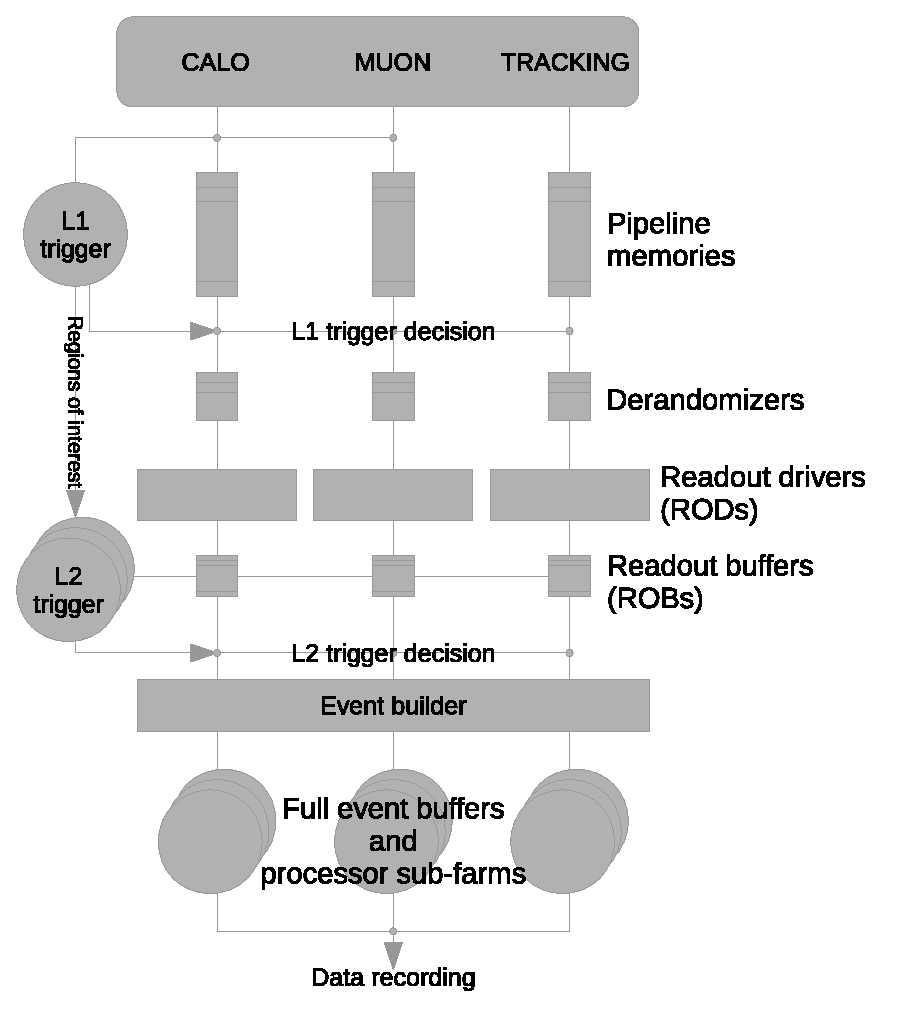
\includegraphics[width=0.6\textwidth]{figures/ATLAS_trigger.eps}
\caption{Diagram of the ATLAS trigger and readout system.}
\label{fig:ATLAS_trigger}}
\end{figure}

The readout system of the ATLAS detector is closely connected with the online trigger system, which consists of two trigger layers (the so-called L1 trigger and L2 trigger), and one event filter~\cite{lib:trigger}. The frequency at which LHC delivers bunch collisions is by design 40 MHz (every 25 ns), although throughout 2011 data taking it was 20 MHz (every 50 ns). It is physically impossible to reconstruct and record every of these 40 millions events per second. And what's more important, only a fraction of these events contain the actual $pp$ collision, so most of the events would be useless even if we managed to record them all. The gradual system of triggers makes an on-the-fly decision whether the event has an actual $pp$ collision or not. The L1 trigger works on the frequency of LHC bunches crossing. This trigger is fully hardware, so it takes a decision in a matter of nanoseconds during the time while the signal from the detectors travels the cables to the readout drivers (RODs). The L1 triggers makes only the rough assumptions about the event, which is it calculates the rough amount of energy deposited in the parts of the calorimeters and muon chambers, and finds so-called "regions of interest" (ROIs), which it passes to the next level trigger, to get a closer look at. The next level trigger is already software based, it is called the L2 trigger, it works on the frequency of 60 KHz and makes its decision while the event is stored in a read-out buffer (ROB). Its output event rate is 5 KHz. The final stage is an event filter which outputs the events at the average rate of 400 Hz. At this rate the events are saved to the output streams. The L2 trigger and the event filter are also collectively called the High Level Trigger (HLT), since they study the event much deeply then the L1 trigger, and work on reconstructed event, rather then the deposited energy, which is what the L1 trigger do. The precision of the L1 trigger is 1 GeV and it only measures the total amount of the deposited $E_{t}$ in the calorimeter towers. The L2 trigger attempts a partial reconstruction of the event in ROIs which are passed down from the L1 trigger as well as track reconstruction, and the event filter does the full event reconstruction in these regions.

The full reconstruction of the filtered event is then done by the large on-site computer farm, and then stored by the use of the data acquisition system (DAQ).
